% === Begin Label Data ===
% ID: 176
% 难度星级: 
% 标签: 
% 备注: 
% 组卷引用次数: 0
% === End  Label Data ===

\begin{problem}{2019}{G}{上海春考卷}{21}{数列}
已知等差数列 $\{a_n\}$ 的公差 $d \in (0, \pi]$, 数列 $\{b_n\}$ 满足 $b_n = \sin(a_n)$, 集合 $S=\{x|x=b_n, n \in \mathbf{N}^*\}$.

（1）若 $a_1=0, d=\dfrac{2\pi}{3}$, 求集合 $S$;

（2）若 $a_1=\dfrac{\pi}{2}$, 求 $d$ 使得集合 $S$ 恰好有两个元素;

（3）若集合 $S$ 恰好有三个元素：$b_{n+T}=b_n, T$ 是不超过 7 的正整数, 求 $T$ 的所有可能的值.
\end{problem}

\begin{solutions}
(1) 因为等差数列 $\{a_n\}$ 的公差 $d\in(0, \pi]$，数列 $\{b_n\}$ 满足 $b_n=\sin(a_n)$，集合 $S=\{x|x=b_n, n\in \mathbb{N}^*\}$.

所以当 $a_1=0, d=\dfrac{2\pi}{3}$，集合 $S=\left\{-\dfrac{\sqrt{3}}{2}, 0, \dfrac{\sqrt{3}}{2}\right\}$.

(2) 因为 $a_1=\dfrac{\pi}{2}$，数列 $\{b_n\}$ 满足 $b_n=\sin(a_n)$，集合 $S=\{x|x=b_n, n\in \mathbb{N}^*\}$ 恰好有两个元素，如图：

根据三角函数线，\circled{1}等差数列 $\{a_n\}$ 的终边落在 $y$ 轴的正负半轴上时，集合 $S$ 恰好有两个元素，此时 $d=\pi$.

\circled{2}$a_1$ 终边落在 $OA$ 上，要使得集合 $S$ 恰好有两个元素，可以使 $a_2, a_3$ 的终边关于 $y$ 轴对称，如图 $OB, OC$，此时 $d=\dfrac{2\pi}{3}$，

综上，$d=\dfrac{2}{3}\pi$ 或者 $d=\pi$.


(3) 
\circled{1}当 $T=3$ 时，$b_{n+3}=b_n$，集合 $S=\{b_1, b_2, b_3\}$，符合题意.

\circled{2}当 $T=4$ 时，$b_{n+4}=b_n$，$\sin(a_n+4d)=\sin a_n, a_n+4d=a_n+2k\pi$，或者 $a_n+4d=2k\pi-a_n$，

等差数列 $\{a_n\}$ 的公差 $d\in(0, \pi]$，故 $a_n+4d=a_n+2k\pi, d=\dfrac{k\pi}{2}$，又 $\therefore k=1, 2$
当 $k=1$ 时满足条件，此时 $S=\{-1, 1, -1\}$.

\begin{center}
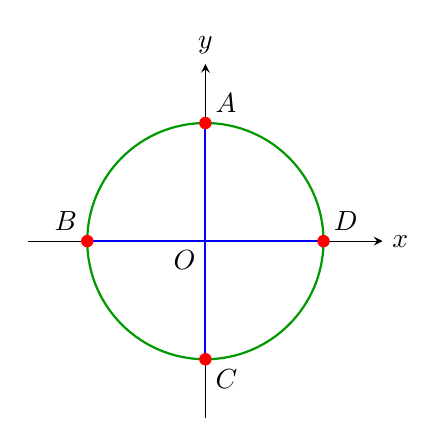
\begin{tikzpicture}[>=stealth, scale=1.5]
    % Draw axes
    \draw[->] (-1.5,0) -- (1.5,0) node[right] {$x$};
    \draw[->] (0,-1.5) -- (0,1.5) node[above] {$y$};
    
    % Draw unit circle
    \draw[green!60!black, thick] (0,0) circle (1);
    
    % Draw radius lines for T=4
    \draw[blue, thick] (0,0) -- (90:1) node[above right, black] {$A$};
    \draw[blue, thick] (0,0) -- (180:1) node[above left, black] {$B$};
    \draw[blue, thick] (0,0) -- (270:1) node[below right, black] {$C$};
    \draw[blue, thick] (0,0) -- (0:1) node[above right, black] {$D$};
    
    % Draw dots
    \foreach \angle in {0, 90, 180, 270}
        \fill[red] (\angle:1) circle (1.5pt);
        
    % Label O
    \node[below left] at (0,0) {$O$};
\end{tikzpicture}
\end{center}

\circled{3}当 $T=5$ 时，$b_{n+5}=b_n$，$\sin(a_n+5d)=\sin a_n, a_n+5d=a_n+2k\pi$，或者 $a_n+5d=2k\pi-a_n$，因为 $d\in(0, \pi]$，故 $k=1, 2$.

当 $k=1$ 时，$S=\left\{\sin\dfrac{\pi}{10}, 1, -\sin\dfrac{\pi}{10}\right\}$ 满足题意.

\circled{4}当 $T=6$ 时，$b_{n+6}=b_n$，$\sin(a_n+6d)=\sin a_n$，

所以 $a_n+6d=a_n+2k\pi$ 或者 $a_n+6d=2k\pi-a_n, d\in(0, \pi]$，故 $k=1, 2, 3$.

当 $k=1$ 时，$S=\left\{\dfrac{\sqrt{3}}{2}, 0, \dfrac{\sqrt{3}}{2}\right\}$，满足题意.

\circled{5}当 $T=7$ 时，$b_{n+7}=b_n$，$\sin(a_n+7d)=\sin a_n=\sin a_n$，所以 $a_n+7d=a_n+2k\pi$，或者 $a_n+7d=2k\pi-a_n, d\in(0, \pi]$，故 $k=1, 2, 3$.

当 $k=1$ 时，因为 $b_1 \sim b_7$ 对应着 3 个正弦值，故必有一个正弦值对应着 3 个点，必然有 $a_m-a_n=2\pi, d=\dfrac{2\pi}{m-n}=\dfrac{2\pi}{7}, m-n=7, m>7$，不符合条件.

当 $k=2$ 时，因为 $b_1 \sim b_7$ 对应着 3 个正弦值，故必有一个正弦值对应着 3 个点，必然有 $a_m-a_n=2\pi, d=\dfrac{2\pi}{m-n}=\dfrac{4\pi}{7}, m-n$ 不是整数，不符合条件.

当 $k=3$ 时，因为 $b_1 \sim b_7$ 对应着 3 个正弦值，故必有一个正弦值对应着 3 个点，必然有 $a_m-a_n=2\pi$ 或者 $4\pi, d=\dfrac{2\pi}{m-n}=\dfrac{6\pi}{7}$，或者 $d=\dfrac{4\pi}{m-n}=\dfrac{6\pi}{7}$，此时，$m-n$ 均不是整数，不符合题意.

\begin{center}
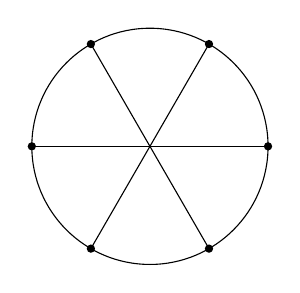
\begin{tikzpicture}[scale=1.5]
    \draw (0,0) circle (1);
    \foreach \i in {0, 60, ..., 300}
        \draw (0,0) -- (\i:1);
    \foreach \i in {0, 60, ..., 300}
        \fill (\i:1) circle (1pt);
\end{tikzpicture}
\quad
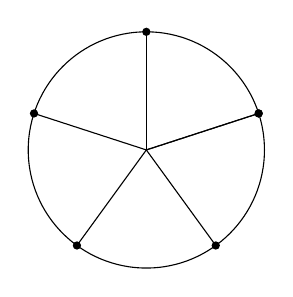
\begin{tikzpicture}[scale=1.5]
    \draw (0,0) circle (1);
    \foreach \i in {18, 90, ..., 378}
        \draw (0,0) -- (\i:1);
    \foreach \i in {18, 90, ..., 378}
        \fill (\i:1) circle (1pt);
\end{tikzpicture}
\quad
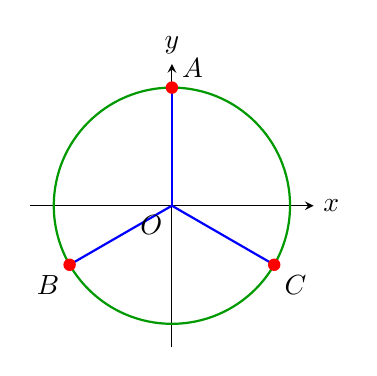
\begin{tikzpicture}[>=stealth, scale=1.5]
    \draw[->] (-1.2,0) -- (1.2,0)  node[right] {$x$};
    \draw[->] (0,-1.2) -- (0,1.2)  node[above] {$y$};
    \draw[green!60!black, thick] (0,0) circle (1);
    \coordinate (A) at (90:1);
    \coordinate (B) at (210:1);
    \coordinate (C) at (330:1);
    \draw[blue, thick] (0,0) -- (A) node[above right, black] {$A$};
    \draw[blue, thick] (0,0) -- (B) node[below left, black] {$B$};
    \draw[blue, thick] (0,0) -- (C) node[below right, black] {$C$};
    \fill[red] (A) circle (1.5pt);
    \fill[red] (B) circle (1.5pt);
    \fill[red] (C) circle (1.5pt);
    \node[below left] at (0,0) {$O$};
\end{tikzpicture}
\end{center}

\begin{center}
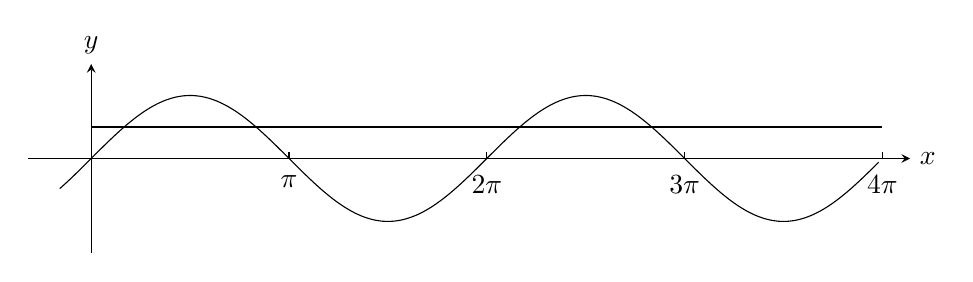
\begin{tikzpicture}[>=stealth, scale=0.8]
    % Sine wave
    \draw[->] (-1,0) -- (13,0) node[right] {$x$};
    \draw[->] (0,-1.5) -- (0,1.5) node[above] {$y$};
    \draw[domain=-0.5:12.5, smooth, samples=100] plot (\x, {sin(\x*180/3.14)});
    \foreach \x/\l in {3.14/\pi, 6.28/2\pi, 9.42/3\pi, 12.56/4\pi}
        \draw (\x, 0) -- (\x, 0.1) node[below=5pt] {$\l$};
    \draw (0,0.5) -- (12.56,0.5);
\end{tikzpicture}
\end{center}

综上，$T=3, 4, 5, 6$.
\end{solutions}